% !TEX TS-program = pdflatex
% !TEX encoding = UTF-8 Unicode

% This is a simple template for a LaTeX document using the "article" class.
% See "book", "report", "letter" for other types of document.

\documentclass[11pt]{article} % use larger type; default would be 10pt

\usepackage[utf8]{inputenc} % set input encoding (not needed with XeLaTeX)

%%% Examples of Article customizations
% These packages are optional, depending whether you want the features they provide.
% See the LaTeX Companion or other references for full information.

%%% PAGE DIMENSIONS
\usepackage{geometry} % to change the page dimensions
\geometry{a4paper} % or letterpaper (US) or a5paper or....
 \geometry{margin=0.5in} % for example, change the margins to 2 inches all round
% \geometry{landscape} % set up the page for landscape
%   read geometry.pdf for detailed page layout information
\usepackage{graphicx} % support the \includegraphics command and options
% \usepackage[parfill]{parskip} % Activate to begin paragraphs with an empty line rather than an indent
%%% PACKAGES
\usepackage{booktabs} % for much better looking tables
\usepackage{array} % for better arrays (eg matrices) in maths
\usepackage{paralist} % very flexible & customisable lists (eg. enumerate/itemize, etc.)
\usepackage{verbatim} % adds environment for commenting out blocks of text & for better verbatim
%\usepackage{subfig} % make it possible to include more than one captioned figure/table in a single float
\usepackage{times}
% These packages are all incorporated in the memoir class to one degree or another...
%\usepackage{biblatex} 
%\bibliography{Essay}
\usepackage{mdframed}
\usepackage{fixltx2e}
\usepackage{hyperref}
%pictures and figures
\usepackage{caption}
\usepackage{subcaption}

\usepackage{listings}
\usepackage{color}
\definecolor{dkgreen}{rgb}{0,0.6,0}
\definecolor{gray}{rgb}{0.5,0.5,0.5}
\definecolor{mauve}{rgb}{0.58,0,0.82}
\lstset{frame=tb,
  language=Python,
  aboveskip=3mm,
  belowskip=3mm,
  showstringspaces=false,
  columns=flexible,
  basicstyle={\small\ttfamily},
  numbers=none,
  numberstyle=\tiny\color{gray},
  keywordstyle=\color{blue},
  commentstyle=\color{dkgreen},
  stringstyle=\color{mauve},
  breaklines=true,
  breakatwhitespace=true
  tabsize=3
}
%%% HEADERS & FOOTERS
\usepackage{fancyhdr} % This should be set AFTER setting up the page geometry
\pagestyle{fancy} % options: empty , plain , fancy
\renewcommand{\headrulewidth}{0pt} % customise the layout...
\lhead{}\chead{}\rhead{}
\lfoot{}\cfoot{\thepage}\rfoot{}

%%% SECTION TITLE APPEARANCE
\usepackage{sectsty}
\allsectionsfont{\sffamily\mdseries\upshape} % (See the fntguide.pdf for font help)
% (This matches ConTeXt defaults)

%%% ToC (table of contents) APPEARANCE
\usepackage[titles,subfigure]{tocloft} % Alter the style of the Table of Contents
\renewcommand{\cftsecfont}{\rmfamily\mdseries\upshape}
\renewcommand{\cftsecpagefont}{\rmfamily\mdseries\upshape} % No bold!

%%% END Article customizations

%%% The "real" document content comes below...

\title{A Comparison and Analysis of Multithreading Language and Library Implementations and Features with Respect to Conway's Game of Life\\Final Year Project}
\author{Edward Michniak 10233252}
\date{} % Activate to display a given date or no date (if empty),
         % otherwise the current date is printed 

\begin{document}
\maketitle
\tableofcontents
\pagebreak
\section{Abstract}
\section{Introduction}
\section{Background Research and Required Knowledge}
\subsection{Life}
%\begin{itemize}
%\item The game at a glance
%\subitem Define a start state
%\subitem Begin automata etc...
%\subitem Moore-neighbourhood
%\item What makes it so interesting?
%\item Why code?
%\subitem "The sheer number of different implementations of this game make it an extremely interesting case study, some languages may be better for one model than an another, an implementation may be possible in one language but not in another!(due to the available features)"
%\end{itemize}

Conway's Game of Life is an example of a {\bf cellular automaton} (CA). This is described \cite[Lesser, Wuensche, 1992 p6]{ref6} as a ``discrete dynamical system which evolves by the iteration of a simple deterministic rule''. When considering constructing a CA there are a few steps one has to follow:
\begin{itemize}
\item Firstly, consider that \emph{time is discrete} and progresses in steps, in this report I will mostly be referring to them as {\bf generations}. A term far more fitting for Conway's Game of Life. 
\item Secondly, an \emph{n-dimensional space} is divided and sectioned into {\bf cells}. This space will have a boundary condition associated with it. I will be implementing the space with an orthogonal toroidal array in 2-dimensions. This means that my boundary conditions would be {\bf cyclic} rather than {\bf absorbing}. {\it figure 1}
\begin{mdframed}
{\bf Extension Note:} However interesting and challenging it may be to implement the Game of Life in 3-D space it is not the focus of this project and for the sake of thread workload scheduling, clarity, and correctness of the result, 2-dimensions is safer and more predictable.
\end{mdframed}
\item Thirdly, each cell has an {\bf attribute} from a limited set of attributes. In the case of Conway's Game of Life, each individual cell can either be dead or alive. Represented in most of my implementations by a 1 or 0. The combined values of all cells in the space are considered to represent the {\bf global state}.
\item Finally, to progress to the next time interval (for instance, to progress from t\textsubscript{0} to t\textsubscript{1}) a {\bf transitional function} is applied to each individual cell using its attribute and the attributes of its {\bf neighbourhood}. Such that, t\textsubscript{1} is the state of the automaton after having the function applied at state t\textsubscript{0}. In this context the Game of Life uses a \emph{Moore-neighbourhood} which consists of the 8 cells surrounding a central cell. However it is worth to note the existence of the \emph{Von Neumann neighbourhood} which pre-dates Moore's implementation. {\it figure 2}
\end{itemize}
\begin{figure}[h]
        \centering
        \begin{subfigure}[h]{0.3\textwidth}
                \centering
                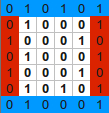
\includegraphics[scale=1]{cyclic}
                \caption{Cyclic boundaries}
                \label{fig:cyclic}
        \end{subfigure}%
        ~ %add desired spacing between images, e. g. ~, \quad, \qquad etc.
          %(or a blank line to force the subfigure onto a new line)
        \begin{subfigure}[h]{0.3\textwidth}
                \centering
                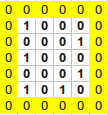
\includegraphics[scale=1]{absorbing}
                \caption{Absorbing boundaries}
                \label{fig:absorb}
        \end{subfigure}
        \caption{Types of boundaries}\label{fig:boundaries}
\end{figure}

\begin{figure}[h]
\centering
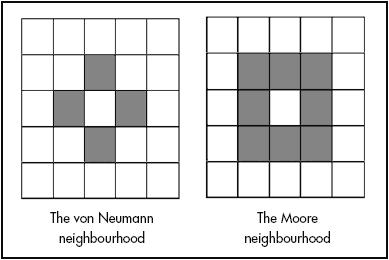
\includegraphics[scale=0.75]{neighbourhood}
\caption{The two types of CA neighbourhood}
\label{fig:neighbourhood}
\end{figure}
Considered by many to be a \emph{zero-player game}, Conway's automaton was first revealed in a 1970 Scientific American article \cite[Gardner]{ref7} where his rules where enumerated and an explanation of how one might play his game was offered. This involved a very laborious method of using a checker board and some two-colour checkers (or something similar), to represent the {\bf global state} and every cells individual attribute. An 8 x 8 grid would require 64 applications of the transitional function to move forward just one generation! Maybe you can begin to see why a computational implementation would be useful?
\subsubsection*{The Laws of Life}
\begin{enumerate}
\item Survivals. Every live cell with two or three neighbouring live cells survives for the next generation.
\item Deaths. Each live cell with four or more neighbour live cells dies (is removed) from overpopulation. Every live cell with one neighbour or none dies from isolation.
\item Births. Each dead cell adjacent to exactly three neighbour live cells--no more, no fewer--is a birth cell. A life is placed on it at the next move. (i.e. the cells attribute is changed) \cite[Gardner, 1970]{ref7}
\end{enumerate}
These laws are going to form the basis of the {\bf transition function} which will be applied to the grid to progress to the next generation.\\
\\What makes the Game of Life so interesting and unique? In the book ``The Game of Life: Cellular Automata'' \cite[Bays, 2010, p1]{ref8} argues that it is ``...the discovery of ``oscillators'' (periodic forms) and ``gliders'' (translating oscillators).'' that are the source of its original fame and interest. These {\it lifeforms} represent a breakthrough in two-dimensional cellular automata and were discovered by mathematician William Gosper in 1970. A prize was offered by John Conway relating to his conjecture that there could be a configuration of the initial state that would constantly promote an ever increasing number of live cells in the global state. Gosper won the prize by demonstrating, and thus coining the term, a glider gun. {\it figure 3}\\
\begin{figure}[h]
\centering
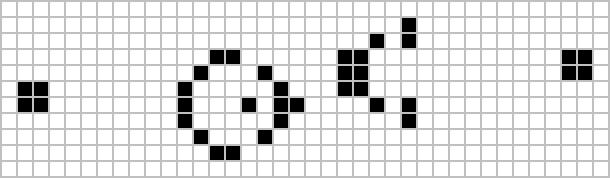
\includegraphics[scale=0.5]{gosper}
\caption{The Gosper Glider Gun}
\label{fig: Gosper}
\end{figure}
\\Why code? Even smallest grid requires a lot of time and effort to move from one generation to the next. Consider the configuration in the grid above and try to process a single generation using a manual method. Boring, repetitive and tedious isn't it? Thankfully computers excel at boring and repetitive tasks that humans find tedious. Also, it's interesting! There's no end to the different implementations that could be written to change some way in which the system executes. Finally, the most common implementation of the Game of Life would involve the allocation of some array structure, and considering the layout of computer memory this is very intuitive and easy to do.\\
\begin{mdframed}
{\bf Extension Note:} There is a vast number of different algorithms that could be implemented. For example, Hashlife, quad-trees, linked-list, bit-stream... An extension could be researched into the relative performance of different algorithms in specific languages and the language features which benefit or hinder execution. My pseudo-algorithm will be outlined later on however I will be focusing on realising and defining parallel points in the program execution and discussing the syntax, semantics and effectiveness for respective implementations. 
\end{mdframed} 
\subsection{Prototype and Experimental Research}
%\begin{itemize}
%\item refactoring the transitional function
%\item Sequential C code?
%\subitem Mention results
%\item Defining parallel points in execution 
%\subitem Reference parallel programming book
%\item Building the abstract pseudo-algorithm for sequential execution
%\item Requirements elicitation? (It has to go somewhere!)
%\subitem Functional and non-functional requirements of language



%\end{itemize}
\subsection{Threads}
\begin{itemize}
\item Von Neumann architecture
\subitem Von Neumann bottleneck?
\item Harvard Architecture
\subitem differences? Bottlnecks?
\item Sequential vs. Threaded
\item Common issues: Consumer-Producer, Cooperation, Race condition, dead lock, live lock.
\item What would happen if we didn't have the synchronisation directives in the code?
\item System kernel? How this effects the handling of threads.
\item Introduction to packages/languages that will be used.
\subitem Briefly explain the differences, look (very quickly) at some syntax.
\item sleep why is this bad?
\item thread states. ready. executing. dead. etc... HOW THE SYSTEM HANDLES THEM!
\subitem how does (generically) a language interface with a systems threads?
\item more needs to be here!
\end{itemize}
\section{Languages, Compilers, and Interpreters}
\begin{itemize}
\item Interesting point: TeX the package used to create documents is a form of compilation.
\item Introduce the languages more formally.
\subitem Is history necessary here? Java history is quite interesting. 
\subitem C99 not supported in windows. Worth mentioning?
\subitem Language type (Functional, procedural/imperative, OO)
\subitem Language features (typing, inheritance, classes, shared objects, evaluation, verbosity)
\item Explain the difference between a compiler and an interpreter (don't forget JIT). 
\subitem Maybe do this during the language introduction? 
\subitem Highlight which language uses which.
\subitem Mention optimisation, take a quick look at some of the C features that offer this (even the deprecated ones: register etc...)
\subitem how do interpreters handle optimisation?
\subitem how can they ever keep up with compiled languages?
\item Recommendations based on research
\subitem Is there one language that offers everything?
\subitem Could a desirable feature be made available to another language/library at little cost?
\end{itemize}
\section{Implementation}
\begin{itemize}
\item Challenges and appropriateness for implementation
\subitem How the programming paradigm (proc, oop, functional){\bf affects the life implementation?} Mainly mention limitations here! (In haskell we can do X, but in C we can do Y blah blah...) Mention typing, inheritance, evaluation, verbosity, classes, shared objects...etc...
\subitem Memory structures? (quad tree, sequential bits, OOP, struct linked list)
\subitem Processing methods (sequential, threaded, more threads, less threads, thread communication?)
\subitem FOR ALL OF THESE MENTION LIMITATIONS AND BENEFITS!
\item Pseudo-Code (both sequential and threaded)
\item UML (both sequential and threaded)
\subitem state diagram showing generation processes
\subitem class diagram for OOP models
\subitem SEQUENCE diagram!! Useful for showing method calls and generation order. Couple with state Diagram
\item Validation technique
\subitem Functional model (Possible haskell, lisp, clojure, ML, Maybe even SaC?!?)
\subitem Original seed grid
\item Program variables!
\subitem How will this effect runtime performance?
\item The Abstract pseudo Algorithm!!
\subitem ``Basic Explanation.txt''
\subsection{C with OpenMP}
\begin{itemize}
\item Language features
\subitem Register
\subitem Inline
\subitem Optimizer compiler
\subitem Precompiler macros
\item Library features
\subitem atomic
\subitem barrier
\subitem master (same as tid == 0)
\subitem single (different to tid == 0, one thread only!)
\subitem parallel
\subitem for (how could this change the code??)
\subitem ordered
\item POI!! Implementing different library directives changes the results drastically.... Why?! Look into trace thread? correction...Linux Trace Tool Kit
\item Does it conform to the abstract routine?
\item shared memory versus private memory implementation. Problems? Results? Terribleness! Include code. EVIDENCE!!
\end{itemize} 

OpenMP is an ``API specification for parallel programming'' ... \cite{ref3}

\subsection{C with PThreads}
\subsection{C++ with Boost}
\subsection{Java with Threads}
\begin{itemize}
\item gcj and javac
\item fork, join, yield, sleep
\item Overheads? Thread creation - compare to C
\item OOP? Threads as an object?
\end{itemize}
\subsection{Pyhton}
\begin{itemize}
\item List comprehension
\item Parallel processing?
\item parallel applications of Map, Reduce, and List Comprehension? Can it be done? Reference Parallel Computing: Architectures, Algorithms, and Applications, C. Bischof et al (Eds.) P203 Implementing Data-Parallel Patterns for Shared Memory with OpenMP GOOD ARTICLE!
\item The other paradigm? Fetching a 3x3 block of cells. Processing them, return the result... 
\end{itemize}
\subsection{C with CUDA}
\section{Analysis}
\subsection{Problems}
\begin{itemize}
\item Should this really be here? It should really be rounded up in each subheading...
\item Optimisations compiler results mess up
\item Functional model learning curve and paradigm shift. 
\item Python - Using functional techniques.
\end{itemize}
\subsection{Syntax and Semantics}
\subsection{Ease of use}
\subsection{Features}
\subsection{Performance}
\subsection{Extensions}
\begin{itemize}
\item Using OOP to recognize patterns and predict movement. I.e. Gliders and inverters.
\end{itemize}
\section{Conclusion}
Some sort of choice based on the most appropriate language.
\section{Bibliography and References}
\nocite{ref1}
\nocite{ref2}
\nocite{ref4}
\nocite{ref5}
\nocite{ref6}
\bibliographystyle{unsrt}
\bibliography{Project.bib}
\section{Appendices}
All the code!! With comments
\end{itemize}
\end{document}